\newpage
\section{Eksamensopgave 10 - Det skrå kast}
\begin{figure}[h!]
    \centering
    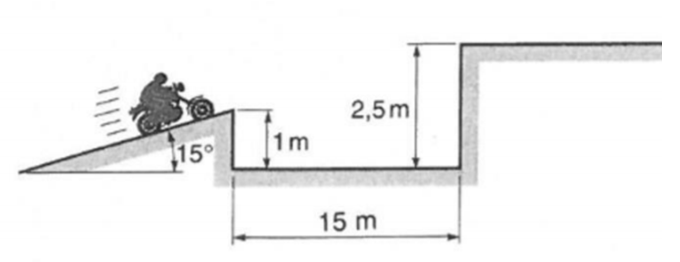
\includegraphics[width=0.5\textwidth]{figures/skrakast.png}
    \caption{Skrå kast opgave}
\end{figure}
\subsection{Hvor lang tid taget springet, når hastigheden er 30m/s}
For at beregne hvor lang tig sprinter tager skal vi først beregne \begin{math}v_{0x}\end{math}\newline
\begin{math}v_{0}\end{math} = Start hastigheden\newline
\begin{math}v_{0x}\end{math} = Start hastigheden på x-aksen\newline
\begin{math}y_{0}\end{math} = Start højde\newline
\begin{math}\alpha\end{math} = Start vinkel\newline
t = tid

\begin{equation*}
    v_{0x}=v_{0}\cdot cos(\alpha)
\end{equation*}
\begin{equation*}
    v_{0x}=30m/s\cdot cos(15^{\circ}) = 28,977 m/s
\end{equation*}
Nu når vi har \begin{math}v_{0x}\end{math} kan vi beregne tiden det tog.
\begin{equation*}
    x=v_{0}\cdot cos(\alpha)\cdot t
\end{equation*}
Nu skal t isoleres ved at dividere med \begin{math}v_{0x}\cdot cos(\alpha)\end{math} på begge sider.
\begin{equation*}
    \frac{x}{v_{0}\cdot \cos(\alpha)}=t
\end{equation*}
\begin{equation*}
    t=\frac{x}{v_{0}\cdot \cos(\alpha)}
\end{equation*}
Fra formlen før ved vi allerede at \begin{math}v_{0}\cdot cos(\alpha) = v_{0x} = 28,977m/s\end{math} og derfor kan formlen omskrives til
\begin{equation*}
    t=\frac{x}{v_{0x}}
\end{equation*}
\begin{equation*}
    t=\frac{15m}{28,977m/s} = 0,518 s
\end{equation*}



\subsection{Skitsér situationen i et koordinatsystem. Indtegn de kræfter som påvirker akrobaten.}


\subsection{Hvor højt passerer han over kanten, hvis farten ved afsættet er 100 km/t?}
Først skal vi omregne 100 km/t til m/s
\begin{equation*}
    v_{0}=\frac{100\cdot 1000}{3600}m/s = 27,78m/s
\end{equation*}
Nu kan vi beregne \begin{math}v_{0x}\end{math} og tiden på samme måde som i opgave a
\begin{equation*}
    v_{0x}=27,78m/s\cdot cos(15^{\circ}) = 26,82 m/s
\end{equation*}
\begin{equation*}
    t=\frac{15m}{26,82m/s} = 0,559 s
\end{equation*}

Nu skal vi beregne y værdien efter 0,559 sekunder med denne formlen
\begin{equation*}
    y_{slut} = -\frac{1}{2}\cdot g\cdot t^{2} + v_{0}\cdot sin(\alpha)\cdot t + y_{0}
\end{equation*}
\begin{equation*}
    y_{slut} = -\frac{1}{2}\cdot 9,82m/s^{2}\cdot 0,559^{2} s + 27,78\cdot sin(15)\cdot 0,559s + 1m = 3,48m
\end{equation*}
Nu har vi den totale højde på y-aksen, derfor skal vi minusse med \begin{math}2,5m - 1m\end{math} da det er højde forskellen, og så kan vi finde højden over kanten
\begin{equation*}
    y_{over} = 3,48m - 1,5m = 1,98m
\end{equation*}
\newpage